\section{Quasi-frozen spin at a periodic lattice}
\label{sec:qfs}

\subsection{Spin motion in electromagnetic fields}

A particle ensemble admits a representation of the spin by a classical vector.
Its dynamics in external electromagnetic fields is described by the
Thomas--Bargmann--Michel--Telegdi (T-BMT)
equation~\cite{Bargmann:1959gz,Fukuyama:2013ioa}. In accordance with the
Ehrenfest theorem, it describes the classical spin motion of a charged particle
with a hypothetical EDM:
\begin{equation}
\begin{aligned}
  \frac{d\vec{S}}{dt} &= \left(\vec{\Omega}_{mdm} + \vec{\Omega}_{edm}\right)\times\vec{S},\\
  \vec{\Omega}_{mdm} &= -\frac{e}{m\gamma}\left\{(\gamma G+1)\vec{B}_{\perp}
     + (1+G)\vec{B}_{\parallel}
     - \left(\gamma G+\frac{\gamma}{\gamma+1}\right)\frac{\vec{\beta}\times\vec{E}}{c}\right\},\\
  \vec{\Omega}_{edm} &= -\frac{e\eta}{2m}\left(\vec{\beta}\times\vec{B}+\frac{\vec{E}}{c}\right),
  \qquad G = \frac{g-2}{2},
\end{aligned}
\label{eq:tbmt}
\end{equation}
where $\gamma$ is the Lorentz factor, $\vec{\beta}$ is the relative velocity,
$c$ is the speed of light, $e$ and $m$ are the particle charge and mass, $G$ is
the magnetic anomaly, $g$ is the gyromagnetic ratio, $\Omega_{mdm}$ and
$\Omega_{edm}$ are the spin precession frequencies due to the magnetic and
electric dipole moments, $\eta$ is a dimensionless coefficient defined by
$d = \eta e\hbar/4mc$, and $\vec{B}=\{B_\perp, B_\parallel\}$ and
$\vec{E}=\{E_\perp, E_\parallel\}$ are the magnetic and electric fields. Since
no elements with a longitudinal magnetic field are used, we set
$B_\parallel = 0$; the longitudinal electric field is neglected as well,
$E_\parallel = 0$, because its contribution is small.

For EDM measurements it is first necessary to compensate the MDM effect. The
simplest approach, initially proposed at BNL~\cite{srEDM:2008_deuteron_proposal}, is the frozen
spin method and uses an all-electric lattice, measuring the spin precession due
to a non-zero EDM in a radial electric field. This method requires
pure-electric optical elements, and the lattice must be designed for and
operated with protons.

An alternative approach is the quasi-frozen spin
concept~\cite{Senichev:2016rez}, based on asynchronous compensation of the spin
precession. The spin vector then oscillates back and forth relative to the
momentum over one period and, as a result, over the full ring.

\subsection{Frozen spin concept}

The frozen spin (FS) method relies on the fact that at a specific, so-called
``magic'' energy the spin precesses in the external fields with the same
frequency as the particle momentum,
$\Omega^{p}_{E,B} = \frac{eE}{m\gamma\beta c} + \frac{eB}{m\gamma}$.
Subtracting this frequency from $\vec{\Omega}_{mdm}$ gives the spin precession
frequency relative to the momentum:
\begin{equation}
  \vec{\Omega}^{p}_{mdm} = \vec{\omega}^{p}_{E} + \vec{\omega}^{p}_{B},
  \label{eq:omega_p}
\end{equation}
where
$\vec{\omega}^{p}_{E} = \frac{e}{m}\left(G-\frac{1}{\gamma^2-1}\right)\frac{\vec{E}\times\vec{\beta}}{c}$
and $\vec{\omega}^{p}_{B} = \frac{e}{m}G\,\vec{B}_{\perp}$ are the
contributions of the electric and magnetic fields. In a purely electrostatic
ring ($\vec{B}=0$) the frozen spin condition $\vec{\omega}^{p}_{E} = 0$ is
satisfied at the magic energy
\begin{equation}
  G - \frac{1}{\gamma_{mag}^2-1} = 0 .
  \label{eq:magic}
\end{equation}
In a ring with both magnetic and electric elements, the frozen spin condition
$\vec{\Omega}^{p}_{mdm}=0$ is achieved by balancing the radial electric field
$E_r$ against the vertical guiding magnetic field $B_v$~\cite{srEDM:2008_deuteron_proposal}:
\begin{equation}
  E_r = \frac{G B_v c\beta\gamma^2}{1-G\beta^2\gamma^2} \approx G B_v c\beta\gamma^2 .
  \label{eq:fs_hybrid}
\end{equation}
A hybrid ring is required for deuterons because their magnetic anomaly is
negative, $G = -0.143$, and condition~\eqref{eq:magic} cannot be satisfied.

It is convenient to introduce the spin tune, i.e., the number of spin
precessions per revolution. In an electrostatic ring the spin tune relative
to the momentum is $\nu_s^E = \omega^p_E/\Omega^p_E$:
\begin{equation}
  \nu_s^E = \left(G-\frac{1}{\gamma^2-1}\right)\gamma\beta^2 ,
  \label{eq:nu_e}
\end{equation}
and in a magnetic field, $\nu_s^B = \omega^p_B/\Omega^p_B$:
\begin{equation}
  \nu_s^B = \gamma G .
  \label{eq:nu_b}
\end{equation}
Thus, the same concept applies to protons and deuterons, but it is realized
with different types of deflectors.

\subsection{Two options of the quasi-frozen spin lattice}

In the NICA ring, an implementation of the FS concept would require a
complete rebuild of the optics. Suppose instead that the spin oscillates in
the horizontal plane around the frozen spin direction with a small amplitude,
$\Phi_s^2 \ll 1$. This can be done with special electric-field elements in the
straight sections, which bring the spin back along the momentum after it has
deviated in the magnetic arc. The EDM signal growth is then reduced by the
factor $J_0(\Phi_s)\approx 1-\Phi_s^2/4$. The deuteron magnetic anomaly
$G=-0.143$ is small, and the spin oscillates around the momentum within half of
the spin phase advance in the magnetic arc,
$\Phi_s = \pi\gamma G/2 \approx 0.25$. Therefore, at the optimal parameters of
the EDM measurement, $\gamma = 1.12$, the effective EDM signal is reduced by
only a few percent.

This gives the essence of the quasi-frozen spin
concept~\cite{Senichev:2016rez}: the spin is not frozen relative to the
momentum but continuously oscillates around an average fixed direction that
coincides with the momentum direction.

Two QFS options exist. In the first one, the magnetic and electric fields are
completely separated in space: the magnetic field acts in the arcs and the
electric field acts in the straight sections, which are realized as
negative-curvature ``reverse'' electrostatic arcs. This option inherits the
drawback of cylindrical electrodes, namely, a whole set of high-order field
nonlinearities. In the second option, a small magnetic field of about
\SI{100}{mT} is added to the spin-aligning E+B elements; it compensates the
Lorentz force of the electric field and makes the elements straight. Such an
E+B element is a Wien filter. The second option is the most appropriate one
for rings not designed specifically for the EDM search, in particular for the
NICA ring with bypass sections, whereas for the Nuclotron, where the free
space is limited, the first option is the baseline.

\subsection{Relative spin motion in QFS}

Let us introduce the QFS concept by examining orbital and spin rotation in a
generalized framework. This approach is based on the dynamics governed by the
Lorentz force for orbital motion and the T-BMT equation~\eqref{eq:tbmt} for
spin precession. The foremost QFS condition that needs to be respected is that
the orbital trajectory remains unperturbed, maintaining a closed orbit
configuration,
\begin{equation}
  \Phi_p^{\mathrm{arc}}+\Phi_{p}^{\mathrm{comp}}=\frac{2\pi}{N},
  \label{eq:QFS_orbital}
\end{equation}
where the index $p$ stands for momentum, $\Phi_p^{\mathrm{arc}}$ and
$\Phi_{p}^{\mathrm{comp}}$ are the total momentum rotations in the arcs and in
the spin-compensator elements, and $N$ is the lattice periodicity. To set up a
lattice suitable for high-energy research, it is essential to employ a pure
magnetic guiding field in the arc, given the limitations of achievable electric
field strengths. Then for a QFS lattice a corresponding spin compensator should
be implemented in the straight section without perturbing the orbit. The
conditions this device should satisfy can be formulated as
$\Phi_p^{\mathrm{arc}} = 2\pi/N$ and $\Phi_{p}^{\mathrm{comp}} = 0$. The second
condition is met by employing both magnetic and electric fields. From
Eq.~\eqref{eq:QFS_orbital}, for a spin-compensation element with both magnetic
and electric fields,
\begin{equation}
  \Phi_{p\mathrm{B}}^{\mathrm{comp}}+\Phi_{p\mathrm{E}}^{\mathrm{comp}} = 0,
\end{equation}
where $\Phi_{p\mathrm{B}}^{\mathrm{comp}}$ and
$\Phi_{p\mathrm{E}}^{\mathrm{comp}}$ are the total momentum rotations in the
magnetic and electric fields of the spin compensator. One can see from the
T-BMT equation~\eqref{eq:tbmt} that the electric field acts on the spin with
maximum effectiveness when it is radial to the momentum. Moreover, it is also
maximally efficient with respect to the momentum rotation, which means
\begin{equation}
  \vec{\Omega}_{p\mathrm{E}}^{\mathrm{max}} = \vec{\Omega}_{p\mathrm{E}_{\perp}}
  =\frac{e}{m \gamma} \frac{\vec{\beta} \times \vec{E}_{\perp}}{c \beta^2}.
\end{equation}

The second QFS condition that needs to be respected is to compensate for the MDM
spin rotation in one period of the ring,
\begin{equation}
  \Phi_s^{\mathrm{arc}}+\Phi_{s}^{\mathrm{comp}}=0,
  \label{eq:QFS_spin}
\end{equation}
where $\Phi_s^{\mathrm{arc}}$ and $\Phi_{s}^{\mathrm{comp}}$ are the total spin
rotations in the arc and in the spin compensator. The spin and orbital rotation
angles are connected by the spin-tune ratios in magnetic and electric fields,
Eqs.~\eqref{eq:nu_b} and~\eqref{eq:nu_e},
\begin{equation}
  \nu_{\mathrm{B}_{\perp}} = \gamma G, \qquad
  \nu_{\mathrm{E}} = \gamma \beta^2 \left(G-\frac{1}{\gamma^{2}-1}\right).
  \label{eq:spin-tune}
\end{equation}
The spin-tune difference is responsible for the compensation effect. In the
pure magnetic arc $\Phi_{s}^{\mathrm{arc}} =
\nu_{\mathrm{B}_{\perp}}\Phi_{p}^{\mathrm{arc}}$, while in the spin compensator
$\Phi_{s\mathrm{B}}^{\mathrm{comp}} =
\nu_{\mathrm{B}_{\perp}}\Phi_{p\mathrm{B}}^{\mathrm{comp}}$ and
$\Phi_{s\mathrm{E}}^{\mathrm{comp}} =
\nu_{\mathrm{E}}\Phi_{p\mathrm{E}}^{\mathrm{comp}}$. Then
Eq.~\eqref{eq:QFS_spin} can be rewritten as
\begin{equation}
\begin{aligned}
  \nu_{\mathrm{B}_{\perp}}\Phi_{p}^{\mathrm{arc}} +
  \bigl(\nu_{\mathrm{B}_{\perp}}\Phi_{p\mathrm{B}}^{\mathrm{comp}} +
  \nu_{\mathrm{E}}\Phi_{p\mathrm{E}}^{\mathrm{comp}} \bigr)
  &=
  \nu_{\mathrm{B}_{\perp}} \bigl(
  \Phi_{p}^{\mathrm{arc}} +
  \Phi_{p\mathrm{B}}^{\mathrm{comp}} \bigr) +
  \nu_{\mathrm{E}}\Phi_{p\mathrm{E}}^{\mathrm{comp}}  = 0.
\end{aligned}
\label{eq:deflection_sum}
\end{equation}
Finally, combining the first and second QFS conditions, the compensator
electric and magnetic field spin-rotation expressions can be obtained:
\begin{equation}
  \Phi_{p\mathrm{E}}^{\mathrm{comp}} = - \Phi_{p\mathrm{B}}^{\mathrm{comp}}
  = {\Phi}_{p}^{\mathrm{arc}}\frac{\gamma^2 G}{G+1}
  =\frac{2\pi}{N}\frac{\gamma^2 G}{G+1}.
  \label{eq:deflection}
\end{equation}
Note that so far no mention was made of the physical structure of the
compensation element, only of the integral features of the presented field
components.

\subsection{Spin compensation element length}

The spin-compensation element length can be calculated as
\begin{equation}
  L = \Phi_{p\mathrm{B}}^{\mathrm{comp}}R_{\mathrm{B}}
    = \Phi_{p\mathrm{E}}^{\mathrm{comp}}R_{\mathrm{E}},
  \label{eq:length}
\end{equation}
where $R_{\mathrm{B}}$ and $R_{\mathrm{E}}$ are the radii of the magnetic and
electric fields, respectively. In general, the net curvature of an element
with combined magnetic and electric fields is
\begin{equation}
  \frac{1}{R} = \frac{1}{R_{\mathrm{B}}}+\frac{1}{R_{\mathrm{E}}}, \quad
  R_{\mathrm{B}}=\frac{B\rho}{B}, \quad
  R_{\mathrm{E}}=\frac{\kappa}{E},
  \label{eq:total_radius}
\end{equation}
where $B\rho = p_{0}/e$ is the magnetic rigidity, $p_{0} = \gamma m\beta c$,
and $\kappa = p_{0}\beta c/e$ is the electrical rigidity. Because the element
must satisfy the zero net orbital distortion condition, the net Lorentz force
must vanish. Therefore, the net curvature is zero, i.e., $1/R = 0$, which
leads to $R_{\mathrm{B}} = -R_{\mathrm{E}}$. The electric field strength
limitation is considerably more stringent than that of the magnetic field.
The compensator length per period can be obtained using
Eqs.~\eqref{eq:deflection} and~\eqref{eq:length}:
\begin{equation}
\begin{aligned}
  L_{\mathrm{min}} = \Phi_{p\mathrm{E}}^{\mathrm{comp}}R_{\mathrm{E}}
  &= \frac{2\pi}{N}\frac{\gamma^2 G}{G+1}\frac{\kappa}{E_{\mathrm{max}}} \\
  &= \frac{2\pi}{N}\frac{G}{G+1}\frac{mc^2}{e}
     \frac{\gamma(\gamma^2-1)}{E_{\mathrm{max}}},
\end{aligned}
\label{eq:length_min}
\end{equation}
where $E_{\mathrm{max}}$ is the maximum electric field, which limits the
minimal achievable length regardless of the particle under study. The total
length $L=L_{\mathrm{min}}^{\mathrm{total}} = N\cdot L_{\mathrm{min}}$ is
independent of the number of periods. Maximum attainable electric fields are
10--\SI{13}{MV/m}~\cite{Kolokolchikov:2026xbv}; this corresponds to a magnetic
field of the order of 70--\SI{90}{mT}.

\subsection{Features of the deuteron and the proton}
\label{sec:qfs-particles}

\subsubsection{Dependence on beam parameters}

The first thing that needs to be accounted for in an efficient analysis of
the spin dynamics is the polarimeter analyzing power. It depends on the beam
energy and has to be maximal to achieve sufficient statistics. The maximum
figure of merit of the polarimeter is reached at a proton beam energy of
\SI{270}{MeV}~\cite{Mcnaughton:1985wyt} and the same is true for
deuterons~\cite{Kurilkin:2010ym}.

Orbital and spin dynamics vary among different types of particles. In the
first place, the deuteron mass-to-charge ratio is twice that of the proton.
In the second place, the anomalous magnetic moments are notably different:
for the proton, $G_{\mathrm{p}} = 1.79$, and for the deuterons,
$G_{\mathrm{d}} = -0.14$. These differences, gathered in
Table~\ref{tab:particles}, call for a tailored approach to each particle
type when designing experiments as well as when analyzing results.

\begin{table}[htbp]
  \centering
  \caption{Particles and experiment parameters.}
  \label{tab:particles}
  \begin{tabular}{lccccc}
    \toprule
    Particle & $A/Z$ & $G$ & $\gamma_{\mathrm{exp}}$ & $E_{\mathrm{exp}}$, MeV/u & $L$, m \\
    \midrule
    Deuteron d & $2$ & $-0.14$ & $1.144$ & $135$ & $53$ \\
    Proton p & $1$ & $1.79$ & $1.289$ & $270$ & $247$ \\
    & & & $1.078$ & $73$ & $53$ \\
    \bottomrule
  \end{tabular}
\end{table}

In a magnetic field, according to Eq.~\eqref{eq:spin-tune}, the direction of
spin precession depends solely on the sign of the anomalous magnetic moment,
i.e., it is independent of energy. However, the magnitude is influenced by both
the energy and the absolute value of the anomalous magnetic moment. For protons, this effect is so important that care must be taken to ensure
that the condition for the spin-vector rotation per arc,
$\gamma G \cdot \Phi_{p}^{\mathrm{arc}} < \pi/2$, is satisfied in order to
preserve the accumulation of the EDM effect for a longitudinally polarized
beam. This implies that QFS lattices only with a periodicity $N=8$ or larger
provide the means to measure the proton EDM.

To be more precise, an EDM measurement under QFS conditions is attenuated
relative to a frozen spin measurement. To first order the attenuation factor
is given by~\cite{Senichev:2023vtx}
\begin{equation}
  J_{0}(\Phi_s^{\mathrm{arc}})=1-\frac{(\Phi_s^{\mathrm{arc}})^2}{4},
  \label{eq:edm_j0}
\end{equation}
where $\Phi_s^{\mathrm{arc}}$ represents the angle associated with the MDM
effect in the arc in one period. For various particle types and structure
periodicities it is cited in Table~\ref{tab:edm}. The maximum periodicity
considered is $N=16$, due to lattice design limitations. The table shows that
the frozen and quasi-frozen spin regimes are practically the same for
deuterons. For protons, only the 16-periodic lattice offers a real opportunity for practical tests of the
QFS approach.

\begin{table}[htbp]
  \centering
  \caption{Parameters of lattices and experiment at a beam energy of
    \SI{270}{MeV}.}
  \label{tab:edm}
  \begin{tabular}{lccc}
    \toprule
    Particle & $N$ & $\Phi_s^{\mathrm{arc}}$, deg & $J_{0}(\Phi_s^{\mathrm{arc}})$ \\
    \midrule
    Deuteron d & $2$ & $-29.45$ & $0.934$ \\
               & $4$ & $-14.72$ & $0.983$ \\
               & $8$ & $-7.36$ & $0.996$ \\
               & $16$ & $-3.68$ & $0.999$ \\
    Proton p & $8$ & $103.83$ & $0.179$ \\
             & $16$ & $51.91$ & $0.795$ \\
    \bottomrule
  \end{tabular}
\end{table}

In electrostatic fields, the analysis of deuteron and proton behaviors is
further complicated by their distinct interactions with the field. For protons,
the direction of spin rotation can depend on the energy, particularly around
the ``magic'' energy, where
$\gamma_{\mathrm{mag}} = \sqrt{(G_{\mathrm{p}}+1)/G_{\mathrm{p}}} = 1.248$
($E_{\mathrm{mag}} = \SI{233}{MeV}$). Nevertheless, the influence on protons is much lower than for deuterons, as
shown in Fig.~\ref{fig:spin-tune}. For
deuterons, on the other hand, there is no equivalent ``magic'' energy, and
their spin rotation behavior remains consistent across the entire energy
range.

\begin{figure}[htbp]
  \centering
  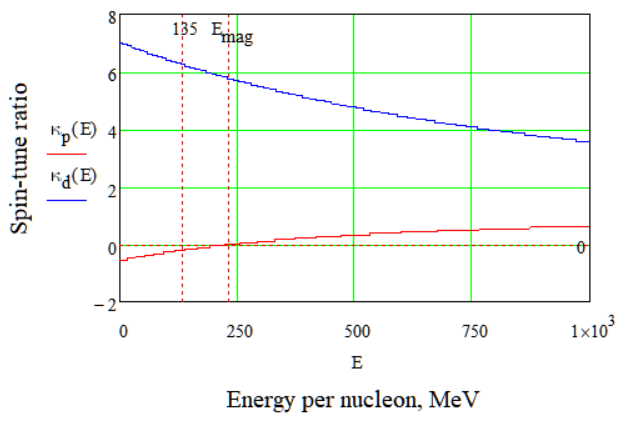
\includegraphics[width=0.58\textwidth]{spin-tune_ratio}
  \caption{Spin-tune ratio
    $\kappa = \nu_{\mathrm{B}_{\perp}}/\nu_{\mathrm{E}}$ for deuteron and
    proton.}
  \label{fig:spin-tune}
\end{figure}

These fundamental differences lead to several important consequences for
lattice construction. Specifically, modifications are necessary to accommodate
both particle types. First, according to Eq.~\eqref{eq:deflection}, the direction of spin rotation
differs between protons and deuterons. This necessitates either switching the
polarity of the spin compensator's fields or rotating it by $\pi$ along the
longitudinal axis. Second, the minimal achievable spin compensator length, as
given by Eq.~\eqref{eq:length_min}, is longer for protons than for deuterons
at the optimal polarimeter energy. This discrepancy can be addressed by
lowering the experimental energy for protons (Fig.~\ref{fig:totallength}). At
a spin compensator length equivalent to that used for deuterons, the proton
energy should be reduced to \SI{73}{MeV}, and the analyzing power decreases by
a factor of 2--3. Third, two viable approaches for arranging additional EM fields are the
implementation of a Wien filter or an electrostatic deflector with a kicker.

\begin{figure}[htbp]
  \centering
  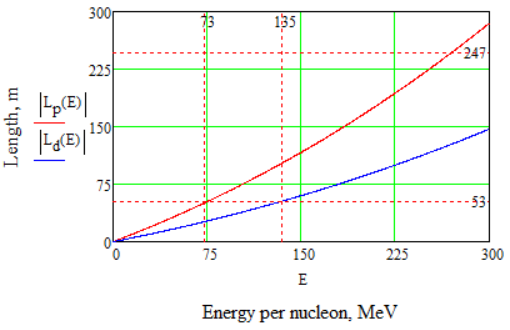
\includegraphics[width=0.58\textwidth]{total_length}
  \caption{Total length of the spin compensator versus energy per nucleon
    required to achieve a QFS lattice for deuteron and proton.}
  \label{fig:totallength}
\end{figure}

\subsubsection{Wien filter}

The Wien filter serves an important function in a particle accelerator,
designed to manipulate spin dynamics without altering the orbital trajectory of
particles by utilizing perpendicular electric and magnetic fields that cancel
each other out, resulting in zero net Lorentz force. As the EDM T-BMT term is
proportional to the Lorentz force, the Wien filter will not exert an EDM force
on the spin vector. It is EDM-transparent. It allows particles to move in a
straight line while enabling a precise correction of their spin orientations,
making it an ideal auxiliary device for experiments requiring spin
manipulation. It provides the conditions to facilitate spin navigation. The
filter's design ensures a net absence of deflection along the beamline,
minimizing additional space requirements in the ring's straight sections and
allowing for a classical sequential arrangement of ring elements.

It is usable for both deuterons and protons; for deuterons, it can be employed
directly at optimal energies, while for protons, the polarity must be switched
or the setup rotated by $\pi$ along the longitudinal axis and used at lower
energies (Figs.~\ref{fig:wf_vector_d}, \ref{fig:wf_vector_p},
\ref{fig:axion_diagram} and~\ref{fig:wien-filter}). This
flexibility allows for freedom in developing methods for studying spin dynamics
across different particle types. Overall, the Wien filter's ability to control
particle spin without perturbing orbital paths makes it an invaluable component
in advanced accelerator experiments.

\begin{figure}[htbp]
  \centering
  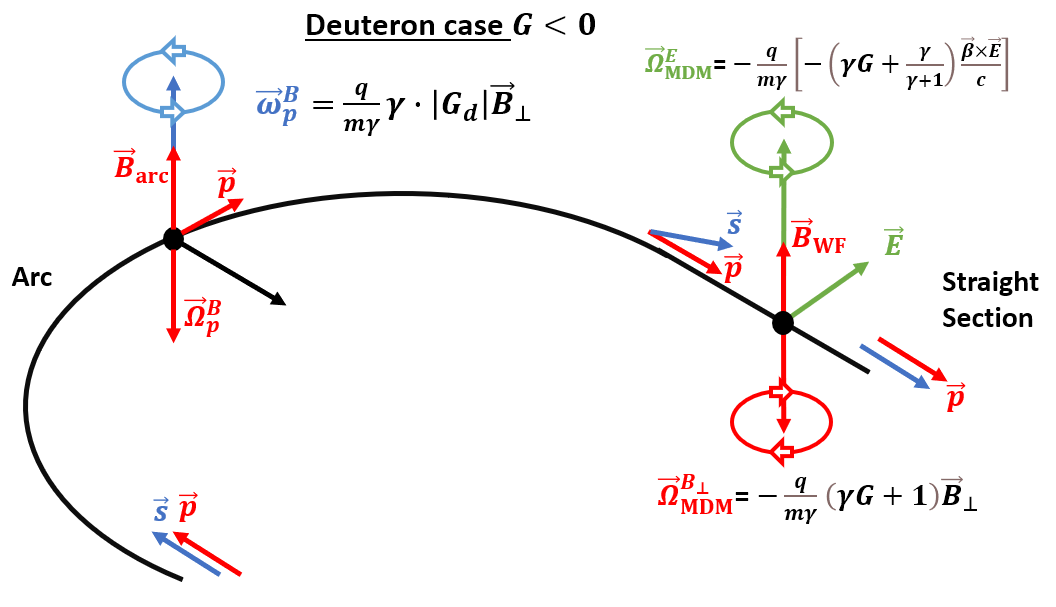
\includegraphics[width=0.92\textwidth]{DeuteronWF_scheme}
  \caption{Vector scheme of the QFS turn with a Wien filter for the deuteron
    case $G<0$.}
  \label{fig:wf_vector_d}
\end{figure}

\begin{figure}[htbp]
  \centering
  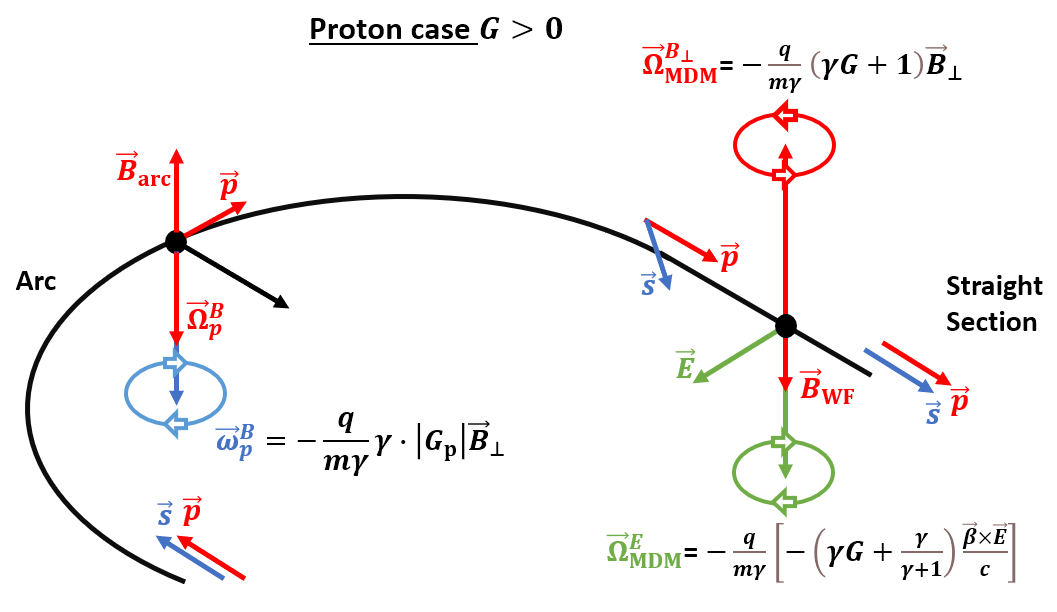
\includegraphics[width=0.92\textwidth]{ProtonWF_scheme}
  \caption{Vector scheme of the QFS turn with a Wien filter for the proton
    case $G>0$.}
  \label{fig:wf_vector_p}
\end{figure}

\begin{figure}[htbp]
  \centering
  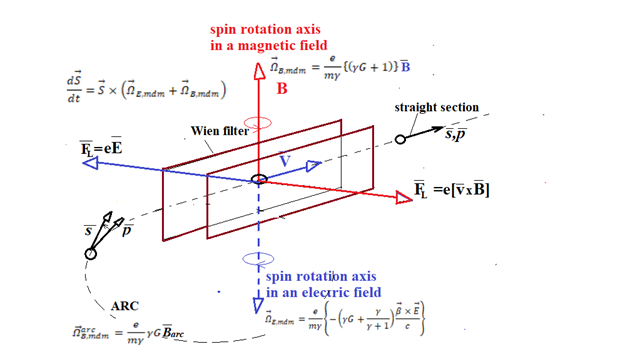
\includegraphics[width=0.88\textwidth]{axion_spin_diagram}
  \caption{Vector diagram of the spin transformation for the deuteron.}
  \label{fig:axion_diagram}
\end{figure}

\begin{figure}[htbp]
  \centering
  \begin{panel}{0.48\textwidth}
    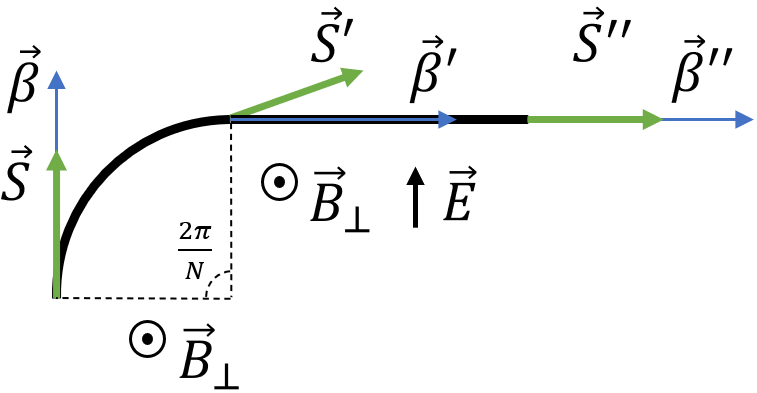
\includegraphics[width=\linewidth]{wien-filter_deuteron}
  \end{panel}\hfill
  \begin{panel}{0.48\textwidth}
    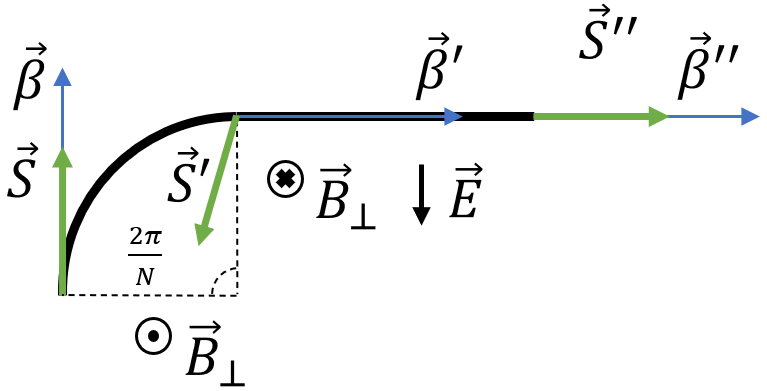
\includegraphics[width=\linewidth]{wien-filter_proton}
  \end{panel}
  \caption{One-period conceptual scheme of a QFS lattice with Wien filters for
    deuterons (a) and protons (b).}
  \label{fig:wien-filter}
\end{figure}

\subsubsection{Electrostatic deflector with kicker}

The pure electrostatic deflector is designed to manipulate particle
trajectories and spin dynamics by creating a radial electric field with a
nonzero curvature. Unlike the Wien filter, this deflector requires an
additional kicker to compensate for orbital deviations, which increases the
overall length of the compensator. This setup is particularly useful for
creating bypass sections in addition to the native straight sections, allowing
for flexible experimental configurations (Fig.~\ref{fig:el-defdeuteron}). However, the distance between the spatial
assignment of equipment should be considered to enable the option with an
independent section. A key challenge is that each
type of particle requires a different curvature, which must be determined at
the outset of lattice design. Despite these complexities, the electrostatic
deflector with kicker offers a robust solution for controlling particle spin
and trajectory.

\begin{figure}[htbp]
  \centering
  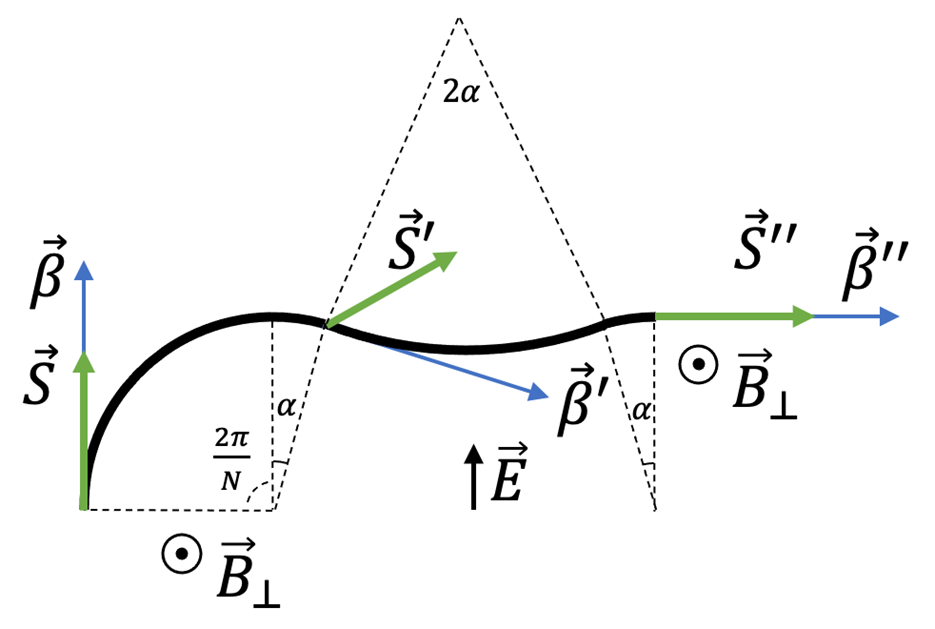
\includegraphics[width=0.7\textwidth]{el-def_deuteron}
  \caption{One-period conceptual scheme of a QFS lattice with an electrostatic
    deflector and a kicker for deuterons.}
  \label{fig:el-defdeuteron}
\end{figure}

\subsection{Further research}

Currently, the proposed energy requirements for EDM studies are set at
\SI{270}{MeV} and lower, but specific conclusions regarding the arc spin
rotation have yet to be drawn. The primary condition is to achieve a momentum
rotation at a specific angle $\Phi_p^{\mathrm{arc}}$ with a corresponding
$\Phi_s^{\mathrm{arc}}$ for the spin. This can be accomplished by carefully selecting the magnetic field integral to ensure precise alignment of
momentum and spin dynamics. To maximize efficiency, the magnetic field should
be as strong as possible to minimize the effective arc length, in consideration
of the unique features of the lattice design. This approach not only optimizes
studies at the current energy range but also opens the possibility for other
polarized or non-polarized beam research at higher energies, potentially
reaching several GeV. The versatility of the QFS setup allows it to be
implemented in various lattice designs, including existing accelerator rings,
thereby facilitating advanced studies at elevated energy ranges.

Wien filters do not affect beam dynamics and influence only the spin motion.
This helps in converting the storage ring into a broadband axion
antenna~\cite{Nikolaev:2022wyi}.

The material of this section has been reported
in~\cite{Kolokolchikov:2026xbv,Senichev:2016rez,Senichev:2023vtx,Senichev:2024qtr,Senichev:2025jqf}.
